\cleardoublepage % memastikan bab baru dimulai di halaman ganjil (kanan)
\chapter{STUDI LITERATUR}
\label{chap:studi-literatur}

% =========================================================
% INSTRUKSI TEMPLATE (dikomentari, tidak dihapus)
\iffalse

\section{Tentang Studi Literatur}
Studi literatur biasanya berisi tentang tinjauan pustaka, landasan teori, dan penelitian-penelitian terdahulu yang relevan dengan topik tugas akhir yang dikerjakan.
Dalam subbab ini, penulis diharapkan dapat menjelaskan:
\begin{enumerate}
  \item Landasan teori yang diperoleh dari literatur yang akan digunakan untuk menyelesaikan persoalan TA;
  \item Pengetahuan tentang kasus yang akan dikaji; dan
  \item Penelitian atau solusi terkait untuk mengetahui posisi persoalan dan berbagai solusi yang memungkinkan untuk diterapkan berdasarkan hasil studi literatur ini.
\end{enumerate}
Jadi, studi literatur ini bukan sekadar rangkuman dari berbagai sumber referensi, tetapi harus diolah dan disajikan secara sistematis sehingga dapat memberikan gambaran yang jelas tentang landasan teori dan penelitian-penelitian terdahulu yang relevan dengan topik tugas akhir.

Penulisan studi literatur yang baik dimulai dari penjelasan tentang kasus yang akan dikaji, kemudian diikuti dengan penjelasan tentang teori-teori yang relevan, dan diakhiri dengan tinjauan terhadap penelitian-penelitian terdahulu yang berkaitan dengan topik tugas akhir.
Misalnya, jika topik tugas akhir adalah tentang masalah klasifikasi biji kopi berdasarkan citra kopi,
penulis dapat memulai dengan menjelaskan terlebih dahulu tentang karakteristik biji kopi, masalah dalam melakukan klasifikasi biji kopi,
kemudian menjelaskan tentang berbagai metode berbasis komputer yang dapat digunakan untuk mengklasifikasikan biji kopi berdasarkan citranya,
metode terbaik yang memungkinkan untuk diterapkan, teori-teori dasar tentang metode tersebut, dan diakhiri dengan tinjauan terhadap penelitian-penelitian terdahulu yang menggunakan metode untuk klasifikasi citra.

Dalam studi literatur, biasanya banyak penjelasan tentang teori-teori yang disertai dengan rumus atau persamaan matematika, gambar, tabel, algoritma, pseudocode, atau kode program.
Oleh karena itu, pada subbab berikut akan dijelaskan beberapa hal teknis terkait format penulisan dokumen tugas akhir.

\section{Format Penulisan Gambar, Tabel, Rumus, dan Kode Program}
Berikut adalah beberapa contoh penulisan gambar, tabel, rumus, dan kode program yang sesuai dengan format penulisan tugas akhir.
\subsection{Penulisan Gambar}
Contoh gambar dapat dilihat pada Gambar \ref{fig:jaringan} dan Gambar \ref{fig:jaringan2}.
Secara vertikal, gambar biasanya diletakkan di bagian atas halaman (\textit{top}) atau di bagian bawah halaman (\textit{bottom}).
Gambar tidak harus diletakkan tepat di tempat gambar tersebut disebutkan pertama kali dalam teks,
tetapi dapat diletakkan di halaman berikutnya jika tidak muat di halaman yang sama. Pada contoh ini, kedua gambar diletakkan di bagian atas halaman
menggunakan opsi \texttt{[t]} pada lingkungan \texttt{figure}, namun pada halaman yang berbeda, meskipun disebutkan di halaman yang sama akibat ruang yang terbatas.

Penyebutan judul gambar dalam teks menggunakan perintah \texttt{ref}, misalnya Gambar \texttt{\\ref\{fig:jaringan\}}.
Gunakan huruf kapital pada kata "Gambar" saat menyebutkan gambar dalam teks.

\begin{figure}[t]
  \caption{Contoh peletakan gambar di bagian atas halaman}
	\label{fig:jaringan}
    	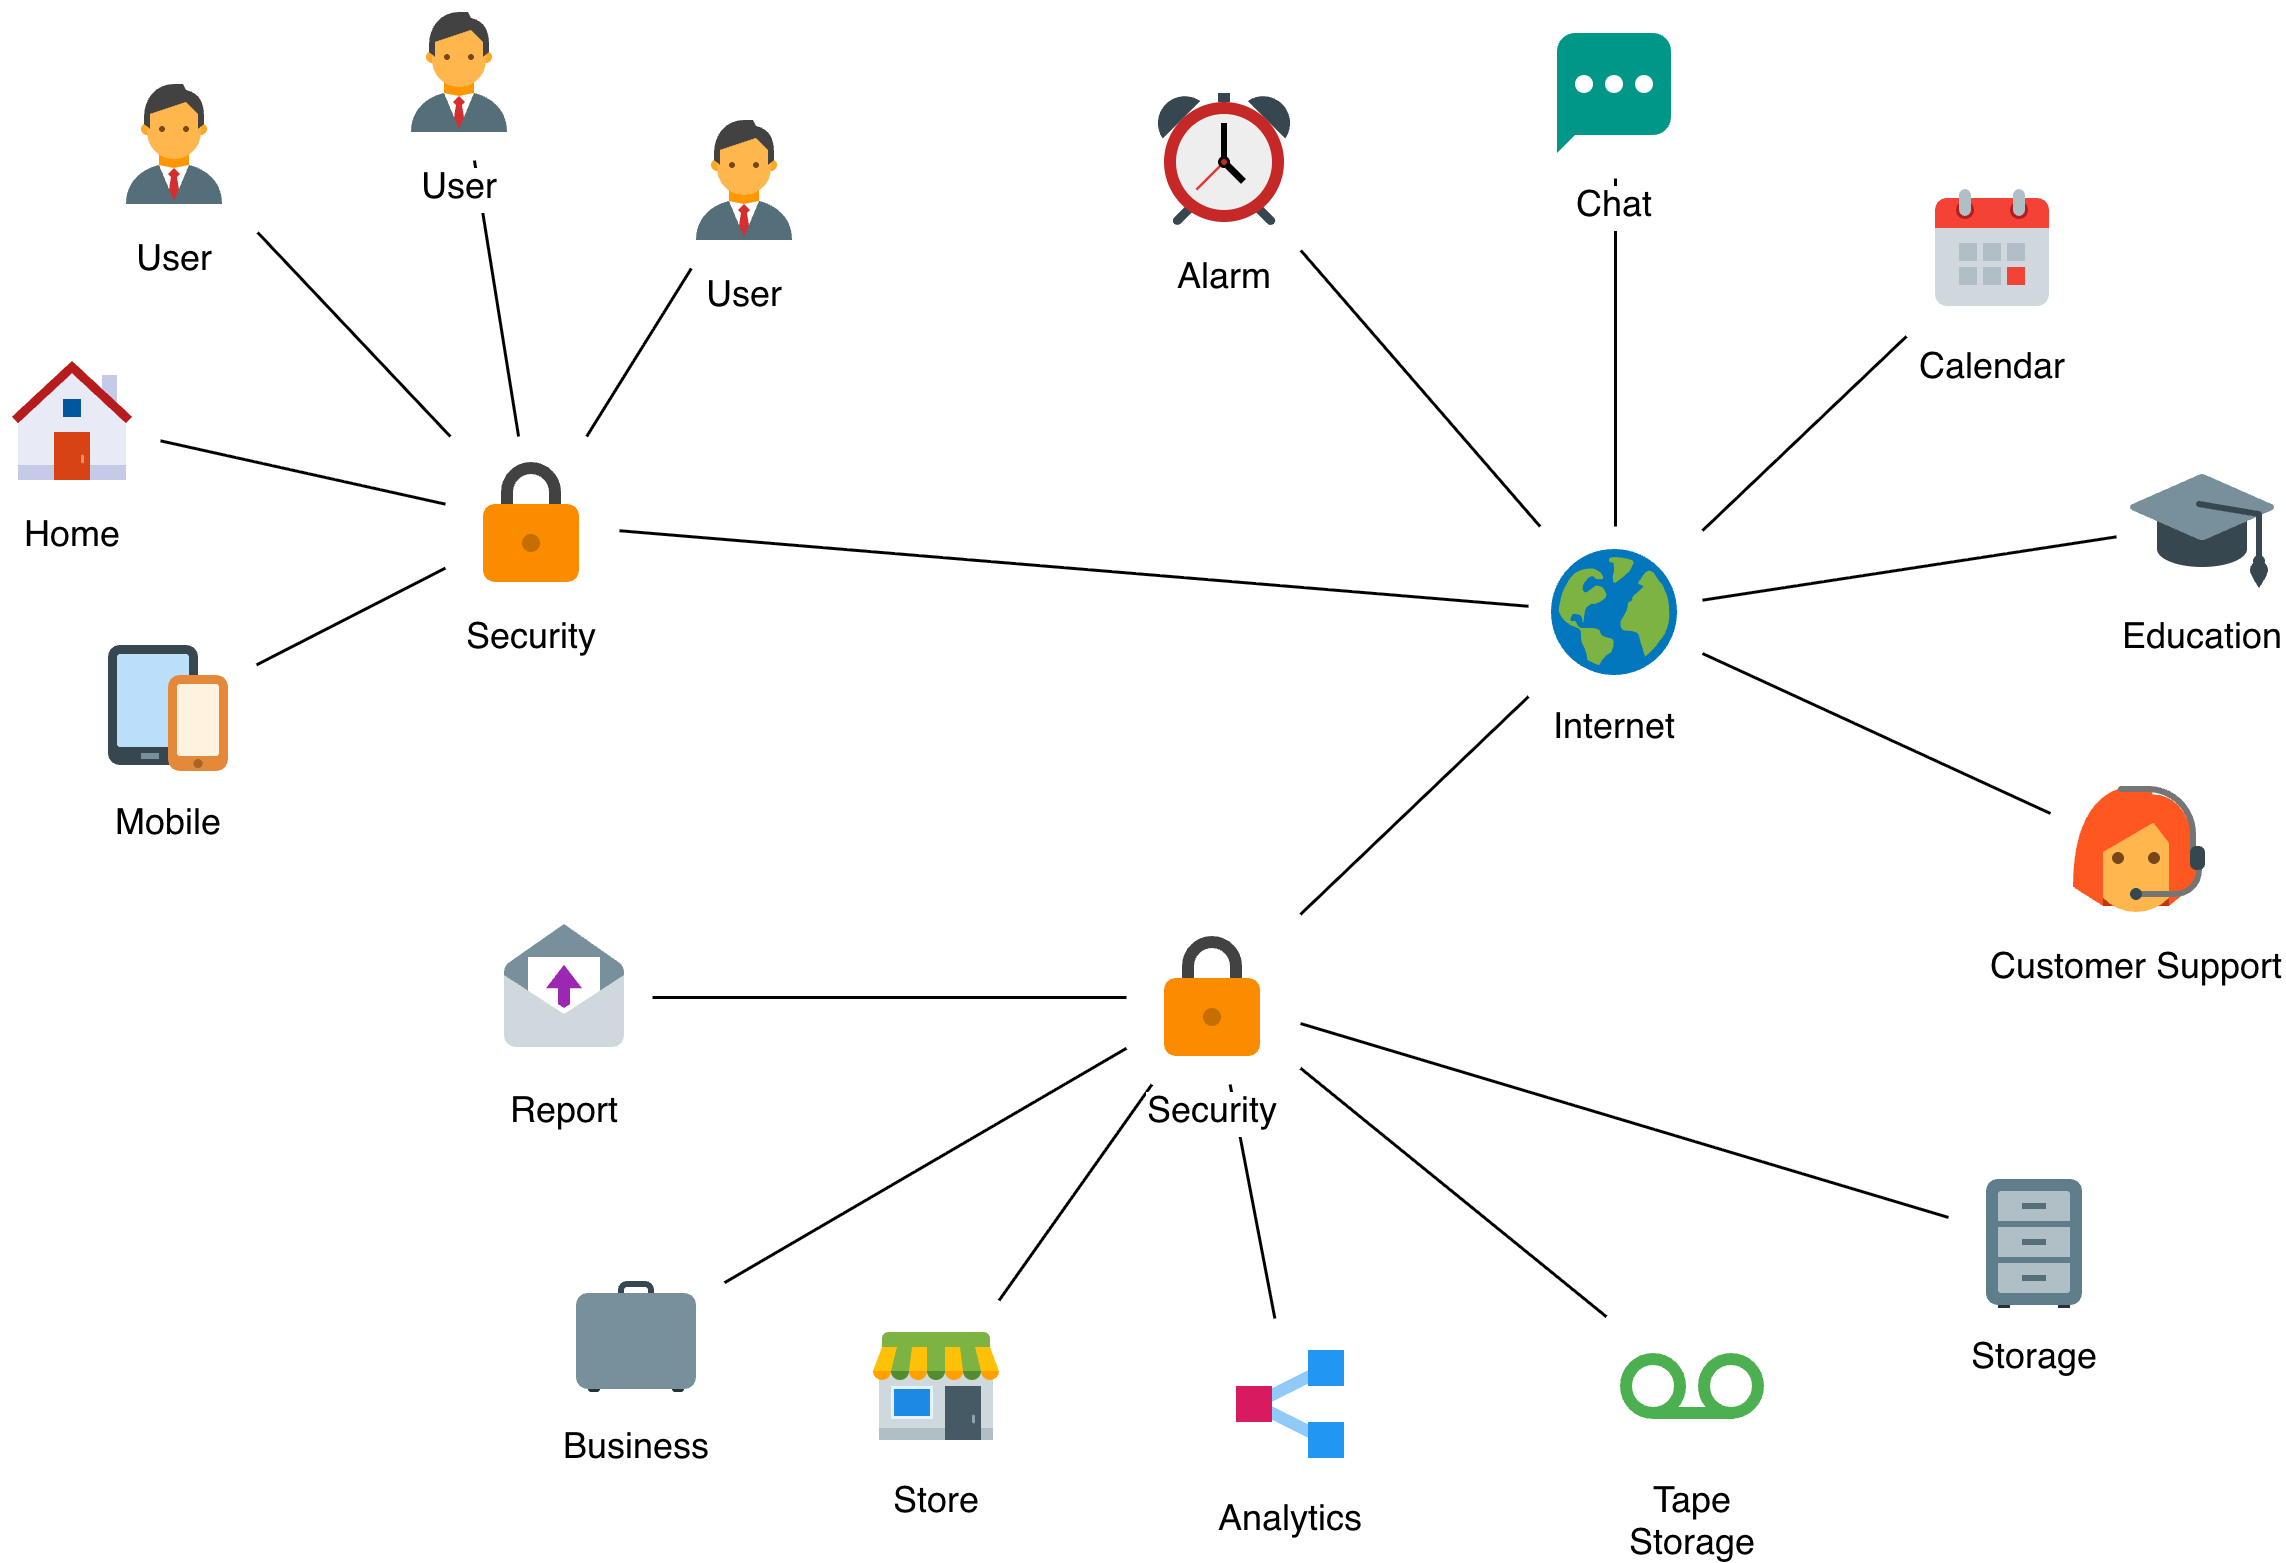
\includegraphics[width=0.7\textwidth]{images/gambar1.png}
\end{figure}

Gambar, grafik, atau ilustrasi harus memiliki keterangan atau judul (\textit{caption}) yang menjelaskan isi gambar tersebut.
Secara horisontal, gambar dan judulnya diposisikan di tengah. Nomor gambar tidak diakhiri tanda baca.
Judul gambar diletakkan di bawah gambar dan ditulis dengan huruf kecil kecuali huruf pertama pada kalimat judul.
Kalimat judul yang panjang dapat ditulis dalam beberapa baris seperti pada Gambar \ref{fig:jaringan2}.

Ukuran gambar yang ditampilkan dapat diatur dengan mengubah nilai \textit{width} dalam sintaks \textit{includegraphics}.
Gambar \ref{fig:jaringan} memiliki lebar 70\% dari lebar teks, sedangkan Gambar \ref{fig:jaringan2} memiliki lebar 90\% dari lebar teks.

\begin{figure}[t]
  \caption{Contoh peletakan gambar dengan judul yang panjang sehingga ditulis dalam beberapa baris}
	\label{fig:jaringan2}
    	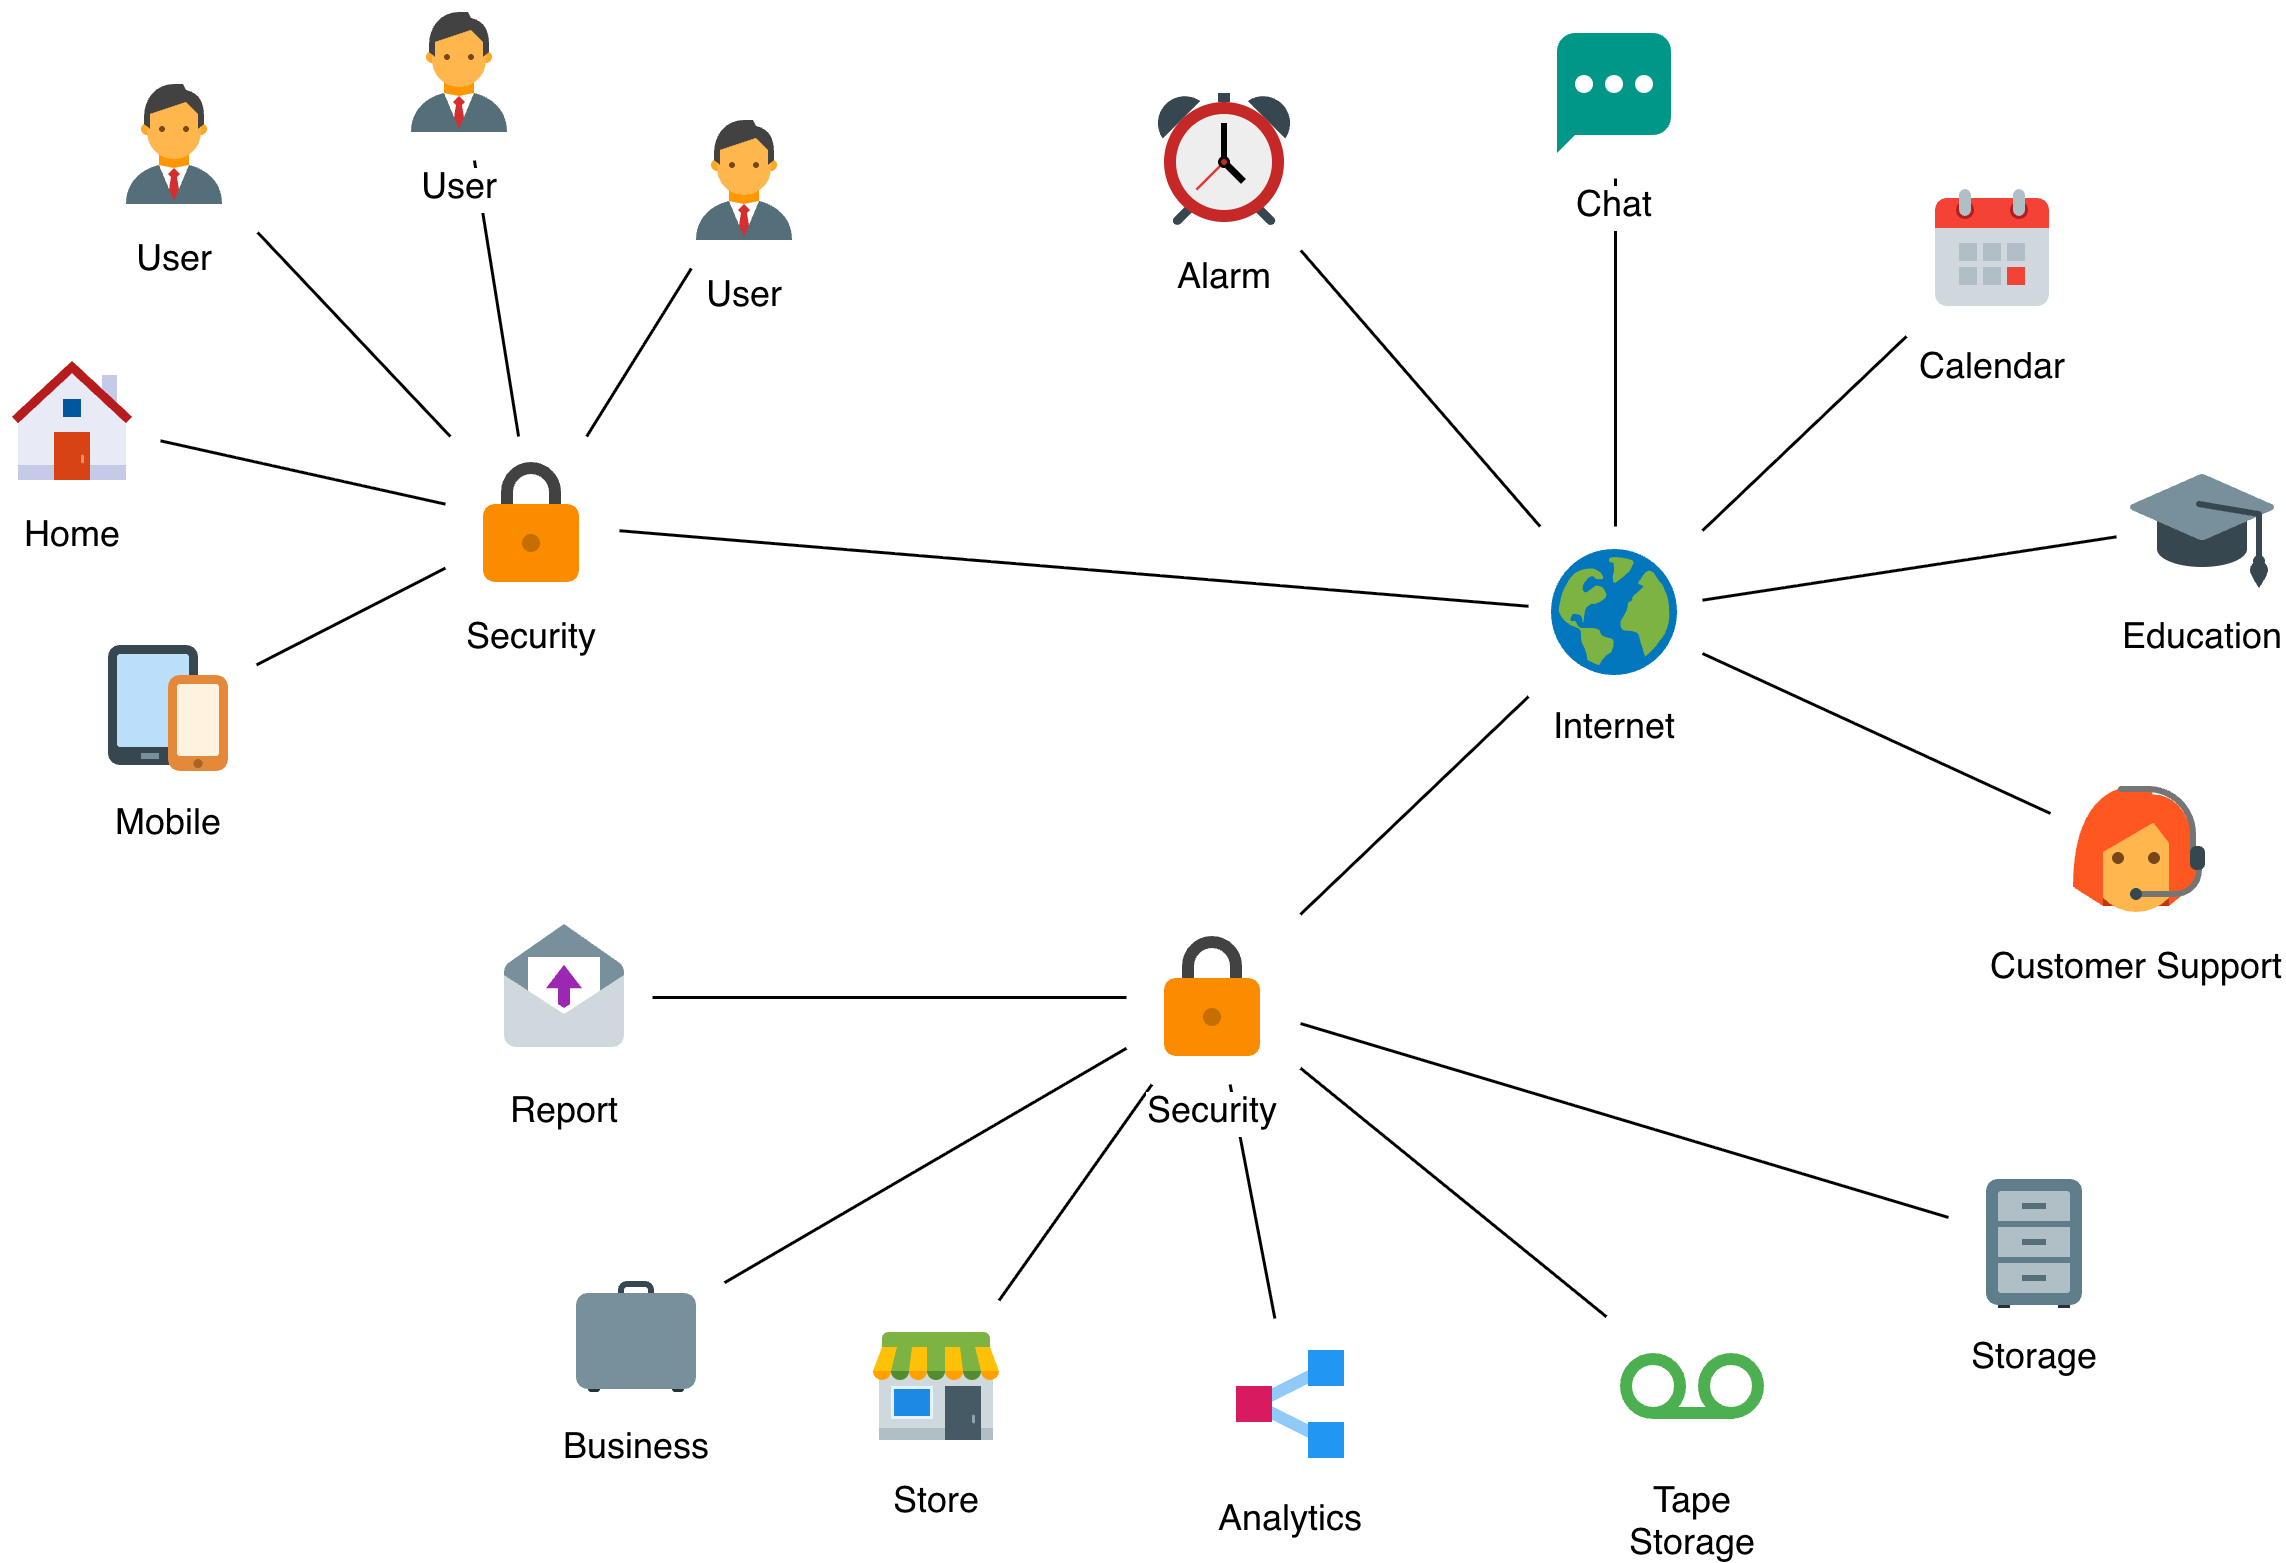
\includegraphics[width=0.9\textwidth]{images/gambar1.png}
\end{figure}

Pastikan gambar yang digunakan memiliki resolusi yang cukup tinggi agar tidak pecah atau buram saat dicetak.
Gambar umumnya tidak tajam dan tulisan tidak jelas atau kabur jika gambar tersebut:
\begin{enumerate}[a.]
  \item diperoleh dari hasil cropping pada suatu halaman buku atau situs web;
  \item hasil pembesaran gambar yang gambar aslinya sebenarnya berukuran kecil; atau
  \item disimpan dalam resolusi kecil
\end{enumerate}
Ketidakjelasan gambar ini dapat dilihat pada garis-garis diagram yang tidak tegas dan tulisan-tulisan dalam gambar yang tampak kabur dan kurang jelas terbaca.

Untuk mendapatkan gambar yang tidak kabur (\textit{blur}), langkah-langkah berikut dapat digunakan:
\begin{enumerate}[(a)]
\item Hindari \textit{screenshot}. Gambar yang didapat di suatu pustaka atau referensi sebaiknya digambar ulang (tidak perlu sama persis), misalnya menggunakan PowerPoint, Canva, Figma, draw.io, atau yang lainnya.
\item Jika diagram atau ilustrasi digambar menggunakan draw.io, saat gambar disimpan ke format PNG atau JPG (\textit{export as}), lakukan \textit{zoom} ke minimal 300\% (\textit{the default value is} 100\%).
\item Jika diagram digambar dengan menggunakan \texttt{PowerPoint} atau aplikasi yang mengolah gambar vektor lainnya, gambar dapat langsung disimpan asalkan resolusinya tinggi.
\end{enumerate}

\subsection{Penulisan Tabel}
Format penulisan tabel hampir sama dengan format penulisan gambar. Bedanya adalah judul tabel diletakkan di atas tabel, bukan di bawah tabel seperti pada gambar.
Ada tabel yang bisa dimuat dalam satu halaman (tabel pendek) dan ada tabel panjang yang yang tidak muat dalam satu halaman. Kedua jenis tabel tersebut disusun dengan cara yang berbeda.
Jika tabel sangat panjang, gunakan paket \textit{longtable} untuk membuat tabel yang dapat terpotong ke halaman berikutnya.
Namun, jika tabel dapat dimuat dalam satu halaman, gunakan lingkungan \textit{table} biasa, tidak menggunakan \textit{longtable}.
Usahakan tabel dapat ditulis dalam satu halaman, tidak terpotong ke halaman berikutnya, jika memungkinkan.

\subsubsection{Penulisan Tabel Pendek}
Contoh tabel pendek dapat dilihat pada Tabel \ref{tab:tabel1}, \ref{tab:tabel2}, dan \ref{tab:tabel3}.
Pada kedua table ini, tabel dan judulnya diposisikan di tengah secara horisontal dan
judul tabel diletakkan di atas tabel. Secara vertikal, tabel sebaiknya diletakkan di bagian atas atau bawah halaman.

Penyebutan judul tabel dalam teks menggunakan perintah \texttt{ref}, misalnya Tabel \ref{tab:tabel1}.
Gunakan huruf kapital pada kata "Tabel" saat menyebutkan tabel dalam teks.

Tabel \ref{tab:tabel1} menggunakan paket \textit{tabularx} untuk mengatur lebar kolom secara fleksibel.
Selain itu, tabel ini juga menggunakan \textit{threeparttable} untuk menambahkan catatan kaki pada tabel
dan opsi \texttt{X} agar lebar kolom fleksibel menyesuaikan lebar tabel.
Catatan kaki pada tabel ini menggunakan perintah \texttt{tablenotes} yang disediakan oleh paket \textit{threeparttable}.
Catatan kaki pada tabel ini menggunakan perintah \texttt{\textbackslash footnotemark} dan \texttt{\textbackslash footnotetext} untuk menambahkan catatan kaki pada tabel.

Tabel \ref{tab:tabel2} menggunakan format standar \texttt{| l | c | r |}.
Tabel \ref{tab:tabel3} menggunakan lebar kolom tetap (\textit{fixed width}) menggunakan \texttt{p\{width\}}.

\begin{table}
  \centering
    \begin{threeparttable}[t]
    \caption{Contoh tabel yang menggunakan \texttt{tabularx} untuk mengatur lebar kolom secara fleksibel.
    Selain itu, tabel ini juga menggunakan \texttt{threeparttable} untuk menambahkan catatan kaki pada tabel
    dan opsi \texttt{X} agar lebar kolom fleksibel menyesuaikan lebar tabel.}
    \label{tab:tabel1}
    \begin{tabularx}{0.6\textwidth}{| c | X| l | r @{}|}
	    \hline
	    No & Nama 	& Satuan 		& Harga \\
	    \hline
	    1 & Buku 	& Exemplar	& 25000 \\
	    2 & Komputer	& Unit		& 2500000 \\
	    3 & Pensil	& Buah		& 118900 \\
	    \hline
	  \end{tabularx}
    \begin{tablenotes}
      \footnotesize
      \item \footnotemark[1]Tabel harga berdasarkan data tahun 2023.
      \item \footnotemark[2]Sumber: \url{https://www.example.com}
    \end{tablenotes}
  \end{threeparttable}
\end{table}

\begin{table}[t]
  \caption{Tabel yang menggunakan format standar \texttt{| l | c | r |}}
  \label{tab:tabel2}
	\begin{tabular}{ | l | c | r | }
	\hline
	Nama 	& Satuan 		& Harga \\
	\hline
	Buku 	& Exemplar	& 25000 \\
	Komputer	& Unit		& 2500000 \\
	Pensil	& Buah		& 118900 \\
	\hline
	\end{tabular}
\end{table}

\begin{table}[t]
  \centering
  \caption{Tabel yang lebar kolomnya dibuat tetap}
  \label{tbl:tabel3}
	\begin{tabular}{  p{0.2\textwidth} | p{0.2\textwidth} | p{0.2\textwidth}  }
	\hline
	\textbf{Nama} 	& \textbf{Satuan} 		& \textbf{Harga} \\
	\hline
	Buku 	& Exemplar	& 25000 \\
	\emph{Komputer}	& Unit		& 2500000 \\
	Pensil	& Buah		& 118900 \\
	\hline
	\end{tabular}
\end{table}

\subsubsection{Mengimpor Tabel dari Berkas Eksternal}

Untuk kerapian penulisan, tabel tidak harus ditulis di dokumen utama. Sebagai contoh, Tabel \ref{tab:tabel4} diimpor dari berkas eksternal \texttt{table/tabel1.tex} menggunakan perintah \texttt{input}.
Dengan demikian, jika tabel tersebut perlu diubah, cukup mengubah pada berkas eksternal tersebut tanpa perlu mengubah pada berkas dokumen utama ini.

\input tables/tabel1.tex

\subsubsection{Tabel yang Sangat Panjang}
Jika tabel terlalu panjang sehingga tidak muat dalam satu halaman, gunakan paket
\textit{longtable} untuk membuat tabel yang dapat terpotong ke halaman berikutnya,
seperti pada Tabel \ref{tab:long}.

\input tables/longtable1.tex

\subsection{Penulisan Rumus atau Persamaan Matematika Menggunakan {\LaTeX} dan Penomorannya}
Contoh rumus matematika dapat ditulis seperti pada Persamaan \ref{eq:contoh1} di bawah ini.
Penomoran persamaan diletakkan di sebelah kanan, dan rumus ditulis dalam mode \textit{display math}.
\begin{equation}
E = mc^2
\label{eq:contoh1}
\end{equation}
\eqcaption{Persamaan Pertama}

Contoh lain penulisan rumus matematika yang lebih kompleks dapat ditulis seperti pada Persamaan \ref{eq:rumus2}.
Perlu diperhatikan bahwa jika rumus terdiri dari beberapa baris, nomor persamaan hanya diletakkan pada baris terakhir, bukan pada setiap baris.
\begin{align}
f(x) &= ax^2 + bx + c \notag \\
f'(x) &= \frac{d}{dx}(ax^2 + bx + c) \notag \\
      &= 2ax + b
      \label{eq:rumus2}
\end{align}
\eqcaption{Persamaan Kedua}

Jika rumus terlalu panjang untuk ditulis dalam satu baris, gunakan lingkungan \textit{multline} seperti pada Persamaan \ref{eq:rumus3} di bawah ini.
\begin{multline}
y = a_0 + a_1x + a_2x^2 + a_3x^3 + a_4x^4 + a_5x^5 + a_6x^6 + a_7x^7 \\
    + a_8x^8 + a_9x^9 + a_{10}x^{10} \label{eq:rumus3}
\end{multline}
\eqcaption{Persamaan Ketiga}

Jika ada penurunan rumus yang terdiri dari beberapa baris, namun tidak memerlukan penomoran pada setiap baris dan tidak masuk di daftar persamaan, gunakan lingkungan \textit{align*}, misalnya:

\begin{align*}
S &= \sum_{i=1}^{n} i^2 \\
  &= 1^2 + 2^2 + 3^2 + \cdots + n^2 \\
  &= \frac{n(n + 1)(2n + 1)}{6}
\intertext{Contoh lainnya adalah rumus untuk mencari nilai rata-rata fungsi $f(x)$ pada interval $[p, q]$:}
\bar{f} &= \frac{1}{q - p} \int_{p}^{q} f(x) \, dx \\
        &= \frac{1}{q - p} \int_{p}^{q} (ax^2 + bx + c) \, dx \\
        &= \frac{1}{q - p} \left[ \frac{a}{3}x^3 + \frac{b}{2}x^2 + cx \right]_p^q \\
        &= \frac{a(q^3 - p^3)}{3(q - p)} + \frac{b(q^2 - p^2)}{2(q - p)} + c \label{eq:rumus4}
\end{align*}

\subsection{Penulisan Kode Program, \textit{Script} atau \textit{Pseudocode}}
Contoh penulisan kode program, \textit{script}, atau \textit{pseudocode} dapat dilihat seperti pada \textit{listing} \ref{lst:binary_iter}.
Gunakan paket \textit{listings} untuk menulis \textit{source code} dalam bahasa pemrograman tertentu.
Kode seperti ini disebut dengan istilah \textit{listing}.
Kode program, \textit{script}, atau \textit{pseudocode} yang relatif pendek dapat ditulis di dalam
dokumen utama. Namun, jika kode programnya sangat panjang, sebaiknya ditulis di berkas terpisah dan diletakkan di lampiran.

\subsection{Penulisan Algoritma}
Contoh penulisan algoritma dapat dilihat pada Algoritma \ref{alg:binary-search}. Ada beberapa paket yang dapat digunakan untuk menulis algoritma,
misalnya \textit{algorithm2e}, \textit{algorithmic}, dan \textit{algpseudocode}.
Pada contoh ini digunakan paket \textit{algorithmic} untuk menulis algoritma. Setiap paket memiliki sintaks yang berbeda-beda.
Oleh karena itu, pelajari dokumentasi paket yang digunakan untuk menulis algoritma.

\input{listings/binary-search-python.tex}

\input{algorithms/binary-search-alg.tex}

\fi
% =========================================================
% AKHIR INSTRUKSI TEMPLATE
% =========================================================

Bab ini menyajikan landasan teori dan tinjauan pustaka yang menjadi fondasi pengembangan modul \emph{People-to-Project} pada platform kolaborasi mahasiswa. Pembahasan dimulai dari konteks domain, yaitu peran mahasiswa dalam kegiatan kolaboratif dan urgensi pencocokan berbasis profil, kemudian dilanjutkan dengan teori-teori teknis yang mendukung perancangan sistem, dan diakhiri dengan tinjauan sistem sejenis yang relevan.

% --- II.1 Mahasiswa dan Kegiatan Kolaboratif ---
\section{Mahasiswa dan Kegiatan Kolaboratif}

Mahasiswa merupakan individu yang berada pada fase penting dalam perkembangan akademik dan profesional. Menurut \textcite{dewey1938}, pembelajaran akan menjadi bermakna apabila mahasiswa terlibat langsung dalam aktivitas yang memberikan pengalaman konkret, karena melalui pengalaman tersebut kemampuan berpikir dan pemecahan masalah dapat berkembang secara lebih mendalam. Pandangan ini menjadi dasar mengapa kegiatan kolaboratif seperti proyek, kompetisi, penelitian bersama, dan magang memiliki nilai strategis bagi perkembangan mahasiswa, bukan sekadar pelengkap kurikulum formal.

\textcite{kolb2014} memperkuat argumen ini melalui teori \emph{experiential learning} yang menjelaskan bahwa mahasiswa mengembangkan pengetahuan secara efektif melalui siklus yang meliputi pengalaman konkret, refleksi, konseptualisasi abstrak, dan eksperimen aktif. Implikasinya, kegiatan kolaboratif yang sesuai dengan kapasitas dan kesiapan mahasiswa akan menghasilkan pengalaman belajar yang lebih bermakna dan berkelanjutan.

Menurut \textcite{roschelle1995}, kolaborasi merupakan aktivitas terkoordinasi yang muncul dari upaya bersama untuk membangun pemahaman yang selaras terhadap suatu permasalahan. \textcite{dillenbourg1999} menambahkan bahwa kolaborasi terjadi ketika individu bekerja bersama dalam keterlibatan yang saling bergantung untuk mencapai tujuan yang telah disepakati.

Namun, akses terhadap banyak pilihan kegiatan yang tidak terstruktur tidak otomatis memudahkan mahasiswa dalam membuat keputusan yang tepat. \textcite{schwartz2004} menjelaskan bahwa ketika individu dihadapkan pada terlalu banyak pilihan tanpa penyaringan yang memadai, mereka cenderung mengalami \emph{choice overload}, yaitu kondisi ketika kelimpahan pilihan justru menghambat pengambilan keputusan dan menurunkan kepuasan terhadap pilihan yang akhirnya dipilih. Dalam konteks mahasiswa yang mencari kegiatan kolaboratif melalui berbagai kanal informal yang tidak terstruktur, kondisi ini berisiko menghasilkan keputusan yang tidak optimal karena informasi tidak dipersonalisasi sesuai profil individu.

Di sisi lain, kemampuan membuat pilihan yang selaras dengan diri sendiri juga bergantung pada kesadaran diri mahasiswa terhadap profil kemampuan dan preferensinya. \textcite{schon1987} menegaskan melalui kerangka \emph{reflective practice} bahwa individu yang mampu merefleksikan kemampuan dan cara kerjanya sendiri dapat membuat pilihan aktivitas yang lebih selaras dengan kapasitas dan tujuan pengembangannya. Tanpa kesadaran diri yang memadai, proses pemilihan kegiatan kolaboratif cenderung bersifat \emph{trial and error} yang tidak efisien dan berisiko menghasilkan ketidakcocokan peran dalam tim.

Relevansi teori-teori di atas terhadap tugas akhir ini adalah jika pembelajaran yang bermakna membutuhkan kegiatan yang sesuai kapasitas dan minat mahasiswa, namun mahasiswa kerap menghadapi kelimpahan informasi yang tidak terstruktur serta keterbatasan kesadaran diri dalam memilih kegiatan, maka mekanisme yang membantu mahasiswa menemukan kegiatan kolaboratif yang cocok dengan profil mereka menjadi kebutuhan nyata. Ini menjadi premis utama yang mendasari pengembangan modul \emph{People-to-Project}.

% --- II.2 Software Development Life Cycle (SDLC) ---
\section{Software Development Life Cycle (SDLC)}

\emph{Software development life cycle} (SDLC) merupakan kerangka proses yang digunakan untuk mengembangkan perangkat lunak secara sistematis, terstruktur, dan dapat dikendalikan. Menurut \textcite{sommerville2016}, SDLC memastikan bahwa setiap tahapan pengembangan mulai dari perumusan kebutuhan hingga pemeliharaan dilakukan secara konsisten untuk menghasilkan sistem yang memenuhi kebutuhan pengguna dan memiliki kualitas yang dapat dipertanggungjawabkan.

\subsection{Waterfall Model}

\emph{Waterfall model} adalah salah satu pendekatan SDLC paling klasik dan banyak digunakan dalam proyek yang memiliki kebutuhan stabil serta ruang lingkup yang terdefinisi dengan jelas. \textcite{sommerville2016} menjelaskan bahwa \emph{waterfall} bekerja secara berurutan (sekuensial), dengan setiap fase harus diselesaikan sebelum beralih ke fase berikutnya. Pendekatan linear ini memberikan struktur yang kuat, dokumentasi yang lengkap, serta kontrol yang baik terhadap alur pengembangan.

\subsection{Requirement Engineering}

\emph{Requirement engineering} adalah proses sistematis untuk menemukan, mendokumentasikan, menganalisis, dan memvalidasi kebutuhan yang harus dipenuhi oleh sistem perangkat lunak. \textcite{sommerville2016} mendefinisikan \emph{requirement engineering} sebagai proses yang membangun pemahaman bersama antara pengembang dan pemangku kepentingan tentang apa yang harus dilakukan sistem. Proses ini merupakan fondasi dari seluruh tahap pengembangan berikutnya.

\textcite{sommerville2016} membedakan dua tingkatan kebutuhan berdasarkan \emph{user requirements} dengan pernyataan dalam bahasa alami yang mendeskripsikan layanan yang diharapkan pengguna dan \emph{system requirements} dengan deskripsi terperinci tentang fungsi dan batasan operasional sistem. Dalam tugas akhir ini, tingkatan tersebut diimplementasikan melalui hierarki tiga lapis yaitu \emph{User Need} (UN), \emph{User Requirement} (UR), dan \emph{Functional Requirement} (FR).

\textcite{sommerville2016} juga membedakan \emph{functional requirements} dan \emph{non-functional requirements}. Pembedaan ini menjadi dasar pengelompokan kebutuhan sistem dalam tugas akhir ini ke dalam FR01--FR14 (fungsional) dan NF01--NF05 (nonfungsional).

% --- II.3 Weighted Scoring Model ---
\section{\emph{Weighted Scoring Model}}

\emph{Weighted Scoring Model} (WSM) merupakan kerangka pengambilan keputusan multi-kriteria yang mengevaluasi sejumlah alternatif secara kuantitatif berdasarkan seperangkat kriteria yang telah diberi bobot. Menurut \textcite{kumar2022}, WSM bekerja efektif untuk pengambilan keputusan multi-kriteria karena setiap alternatif dievaluasi secara numerik terhadap setiap kriteria yang telah diberi bobot sehingga menghasilkan proses penilaian yang transparan dan dapat direplikasi.

Secara operasional, setiap alternatif diberi nilai pada setiap kriteria dengan skala tertentu, kemudian nilai tersebut dikalikan bobot kriteria yang bersangkutan. Hasil perkalian untuk seluruh kriteria dijumlahkan menjadi satu skor total per alternatif; alternatif dengan skor total tertinggi merupakan pilihan yang direkomendasikan. Pendekatan ini memungkinkan perbandingan yang adil antaralternatif meskipun kriteria memiliki tingkat kepentingan yang berbeda-beda. Dalam tugas akhir ini, WSM diterapkan pada Bab III untuk memilih paradigma sistem rekomendasi yang sesuai dengan karakteristik permasalahan pencarian kegiatan kolaboratif mahasiswa.

% --- II.4 Sistem Rekomendasi dan Pencocokan ---
\section{Sistem Rekomendasi dan Pencocokan}

Menurut \textcite{ricci2011}, sistem rekomendasi berfungsi sebagai alat pendukung keputusan yang menyaring informasi dan menampilkan pilihan yang paling sesuai bagi pengguna ketika mereka menghadapi banyak opsi. \textcite{burke2002} menjelaskan pencocokan sebagai inti dari sistem rekomendasi karena proses ini menentukan apakah sebuah item relevan bagi profil pengguna.

\subsection{\emph{Person Job Fit Theory}}

Konsep \emph{person job fit} menjelaskan tingkat kesesuaian antara karakteristik individu dan tuntutan suatu pekerjaan atau aktivitas. Menurut \textcite{kristofbrown2005}, \emph{person job fit} terjadi ketika kemampuan, keterampilan, minat, serta preferensi individu sejalan dengan kebutuhan, tugas, dan karakteristik suatu pekerjaan. Semakin tinggi tingkat kecocokan ini, semakin besar kemungkinan seseorang akan menunjukkan performa yang baik dan mencapai kepuasan dalam pekerjaannya.

Teori ini secara langsung mendasari desain dimensi pencocokan dalam modul \emph{People-to-Project}. Atribut mahasiswa (minat, keterampilan, preferensi peran, gaya kerja) dipadankan dengan kebutuhan kegiatan kolaboratif secara kuantitatif.

Dalam penerapannya, \textcite{langgeng2021} merinci dua dimensi kecocokan tersebut secara lebih operasional. \emph{Demands-Abilities Fit} (DA Fit) mengukur sejauh mana kemampuan dan keterampilan teknis individu memenuhi tuntutan suatu aktivitas, sedangkan \emph{Needs-Supplies Fit} (NS Fit) mengukur sejauh mana aktivitas tersebut memenuhi kebutuhan psikologis, minat, dan preferensi individu. Kedua dimensi bersifat komplementer dan tidak dapat saling menggantikan: seseorang dapat memiliki kemampuan teknis yang memadai namun tidak merasa puas apabila minat dan preferensinya tidak terpenuhi, atau sebaliknya.

Selain kemampuan dan minat, kecocokan dalam kegiatan kolaboratif juga dipengaruhi oleh kesesuaian peran dan gaya kerja antaranggota. \textcite{burke2019} menganalisis taksonomi peran fungsional Benne dan Sheats yang mengklasifikasikan peran anggota kelompok ke dalam tiga kelompok besar: \emph{task roles} yang berfokus pada penyelesaian tugas, \emph{building and maintenance roles} yang berfokus pada pemeliharaan dinamika kelompok, dan peran individual. Pemahaman tentang kecenderungan peran menjadi faktor penting dalam menentukan kecocokan antaranggota tim kolaboratif.

Dari sisi gaya kerja, \textcite{stum2009} menjelaskan teori \emph{Adaption-Innovation} Kirton yang menempatkan individu pada spektrum antara dua kutub kognitif: \emph{Adaptor}, yang cenderung bekerja dalam kerangka terstruktur dengan prosedur yang telah ditetapkan, dan \emph{Innovator}, yang lebih nyaman dengan pendekatan terbuka dan eksploratif tanpa batasan prosedural yang ketat. Perbedaan gaya kerja ini secara langsung memengaruhi kenyamanan dan produktivitas kolaborasi sehingga relevan sebagai salah satu dimensi dalam pencocokan kegiatan kolaboratif.

\subsection{Vocational Interests Theory (Holland)}

\textcite{holland1959} menjelaskan bahwa individu memiliki kecenderungan minat dan preferensi aktivitas tertentu yang dapat digunakan untuk memprediksi kecocokan mereka terhadap suatu lingkungan kerja. Model ini dikenal sebagai RIASEC: \emph{Realistic, Investigative, Artistic, Social, Enterprising}, dan \emph{Conventional}. Relevansinya adalah sebagai justifikasi penggunaan \emph{interest type} sebagai salah satu dimensi berbobot dalam mekanisme pencocokan.

\subsection{Paradigma Sistem Rekomendasi}

Sistem rekomendasi dapat dikategorikan ke dalam tiga paradigma utama berdasarkan mekanisme yang digunakan untuk menghasilkan rekomendasi \autocite{ricci2011}. Pemahaman terhadap ketiga paradigma ini menjadi landasan dalam menentukan pendekatan yang paling sesuai untuk diterapkan pada modul \emph{People-to-Project}.

\emph{Collaborative Filtering} (CF) merekomendasikan item berdasarkan pola perilaku dan preferensi pengguna lain yang memiliki karakteristik serupa. \textcite{adomavicius2005} menjelaskan bahwa pendekatan ini membutuhkan data historis interaksi pengguna dalam jumlah yang cukup untuk menghasilkan rekomendasi yang akurat sehingga rentan terhadap masalah \emph{cold start} pada platform baru yang belum memiliki data historis memadai.

\emph{Content-Based Filtering} (CBF) merekomendasikan item berdasarkan kesamaan antara atribut profil pengguna dan atribut item yang tersedia. Pendekatan ini lebih independen dari riwayat interaksi dibandingkan CF, namun masih memerlukan histori preferensi pengguna untuk membangun representasi profil yang akurat \autocite{ricci2011}.

\emph{Knowledge-Based Recommendation} (KBR) merekomendasikan item berdasarkan pengetahuan eksplisit tentang atribut pengguna dan aturan domain, tanpa memerlukan riwayat interaksi. \textcite{burke2002} menjelaskan bahwa pendekatan ini sangat efektif untuk mengatasi masalah \emph{cold start} karena tidak bergantung pada data perilaku historis, melainkan pada spesifikasi kebutuhan dan karakteristik pengguna yang dinyatakan secara eksplisit.

\subsection{\emph{Rule Based Matching}}

Menurut \textcite{jackson1999}, \emph{rule based matching} adalah sistem berbasis aturan yang bekerja dengan prinsip \emph{if-then rules}. \textcite{burke2002} menjelaskan bahwa pendekatan ini termasuk dalam kategori \emph{knowledge based recommender systems}. Kelebihannya adalah tingkat interpretabilitas yang tinggi \autocite{russell2010}, namun menjadi kurang fleksibel ketika jumlah aturan meningkat. Keterbatasan ini menjadi motivasi pengembangan \emph{affinity based matching}.

\subsection{\emph{Affinity Based Matching}}

\emph{Affinity based matching} merupakan pengembangan dari \emph{rule based matching} yang menambahkan mekanisme penilaian kuantitatif. Pendekatan ini memberikan \emph{affinity score} berupa nilai numerik yang merepresentasikan tingkat kecocokan berdasarkan bobot atribut yang relevan.

\textcite{burke2002} menjelaskan bahwa \emph{knowledge based scoring} dapat diperluas dengan mekanisme pembobotan. \textcite{felfernig2014} menyatakan bahwa rekomendasi dapat dihitung berdasarkan tingkat pemenuhan serangkaian \emph{constraints} berbobot. \textcite{adomavicius2011} memperkuat dasar konseptual ini dengan menekankan bahwa relevansi antara pengguna dan item dapat dievaluasi melalui pendekatan multidimensional yang menggabungkan berbagai atribut dan bobotnya. Pendekatan pembobotan multi-atribut ini juga memiliki dukungan empiris: \textcite{sarsenbay2025} menunjukkan bahwa \emph{pipeline} rekomendasi yang menggabungkan beberapa kelompok atribut psikologis dan kompetensi secara berbobot menghasilkan rekomendasi yang lebih \emph{robust} dibandingkan pendekatan atribut tunggal.

\subsection{\emph{Rank Order Centroid}}

\emph{Rank Order Centroid} (ROC) adalah metode \emph{rank-based surrogate weighting} dalam literatur MCDA yang digunakan untuk mengonversi urutan preferensi antaratribut (\emph{ranking}) menjadi bobot kardinal yang dapat langsung digunakan dalam model pembobotan. Metode ini bekerja dengan asumsi bahwa urutan dominasi antaratribut telah diketahui, namun rasio bobot antaratribut belum dapat ditentukan secara tepat melalui instrumen langsung.

\textcite{hatefi2023} menunjukkan melalui simulasi komprehensif bahwa ROC secara konsisten mengungguli metode \emph{rank-based} lain seperti \emph{Rank Sum} dan \emph{Rank Reciprocal} dalam berbagai skenario pengambilan keputusan. Bobot ROC untuk atribut pada peringkat ke-$i$ dari $n$ atribut diformulasikan pada Persamaan~\ref{eq:roc-litrev} berikut.

\begin{equation}
  w_i = \frac{1}{n} \sum_{k=i}^{n} \frac{1}{k}
  \label{eq:roc-litrev}
  \eqcaption{Bobot \emph{Rank Order Centroid} (ROC)}
\end{equation}

Dengan rumusan ini, atribut pada peringkat tertinggi (peringkat 1) memperoleh bobot terbesar, dan bobot menurun secara konsisten seiring bertambahnya peringkat. Dalam tugas akhir ini, ROC digunakan untuk mengonversi urutan dominasi atribut yang diperoleh dari hasil survei menjadi bobot kardinal yang diterapkan pada kedua sub-algoritma \emph{AffinityEngine}.

\subsection{\emph{Explainability} dalam Sistem Rekomendasi}

\textcite{tintarev2007} mendefinisikan \emph{explanation} dalam konteks sistem rekomendasi sebagai fitur yang menjelaskan kepada pengguna mengapa sebuah item tertentu direkomendasikan. \textcite{burke2002} mencatat bahwa \emph{knowledge based recommender systems} secara inheren memiliki keunggulan interpretabilitas karena keputusan didasarkan pada atribut yang eksplisit.

Dalam sistem yang dikembangkan, \emph{explainability} diimplementasikan melalui FR07, yaitu kemampuan menampilkan \emph{breakdown} skor per dimensi pencocokan (minat, keterampilan, preferensi peran, gaya kerja, dan komitmen waktu) untuk setiap kegiatan yang direkomendasikan.

% --- II.4 Tinjauan Sistem Sejenis ---
\section{Tinjauan Sistem Sejenis}

Tinjauan terhadap sistem sejenis dilakukan untuk mengidentifikasi solusi yang sudah ada, memahami pendekatan yang digunakan, serta menentukan \emph{gap} yang menjadi justifikasi pengembangan sistem baru. Perbandingan beberapa platform yang relevan dengan modul \emph{People-to-Project} yang dikembangkan dalam penelitian ini disajikan pada Tabel~\ref{tab:tinjauan-sistem}.

\begin{table}[H]
  \centering
  \caption{Perbandingan Sistem Sejenis}
  \label{tab:tinjauan-sistem}
  \begin{tabularx}{\textwidth}{p{2.2cm} p{2.8cm} p{3cm} X}
    \toprule
    \textbf{Platform} & \textbf{Fokus} & \textbf{Mekanisme Pencocokan} & \textbf{Kelemahan} \\
    \midrule
    LinkedIn & Jejaring profesional \& rekrutmen & Koneksi manual berbasis riwayat kerja & Tidak dirancang untuk konteks kolaborasi mahasiswa, tidak ada rekomendasi berbasis atribut multidimensi \\
    \midrule
    CATME TeamMaker & Pembentukan tim di kelas formal & \emph{Rule-based} berbasis instruktur & Terbatas pada konteks kelas, tidak mendukung pencarian mitra individual \\
    \midrule
    Kaggle Team Up & Pencarian mitra kompetisi \emph{data science} & Manual, berbasis skor kompetisi & Tidak ada rekomendasi otomatis, terbatas pada domain \emph{data science} \\
    \midrule
    Piazza & Pencarian mitra sesama mahasiswa sekelas & Manual berbasis pengumuman & Pencocokan tidak otomatis, terbatas pada satu mata kuliah \\
    \bottomrule
  \end{tabularx}
\end{table}

Berdasarkan tinjauan di atas, dapat diidentifikasi beberapa \emph{gap} yang belum terjawab oleh sistem yang ada: (1) tidak ada platform yang secara khusus menyediakan rekomendasi kegiatan kolaboratif otomatis berbasis atribut profil multidimensi untuk mahasiswa, (2) platform yang ada umumnya bersifat manual atau terbatas pada domain dan konteks tertentu, dan (3) tidak ada mekanisme yang secara eksplisit menghitung dan menampilkan skor kecocokan antarmahasiswa. \emph{Gap} inilah yang menjadi justifikasi pengembangan modul \emph{People-to-Project} dalam penelitian ini.
